\documentclass{standalone}
\usepackage{tikz}
\usepackage{ctex,siunitx}
\usepackage{tkz-euclide}
\usepackage{amsmath}
\usetikzlibrary{patterns, calc}
\usetikzlibrary {decorations.pathmorphing, decorations.pathreplacing, decorations.shapes,}
\begin{document}
\small
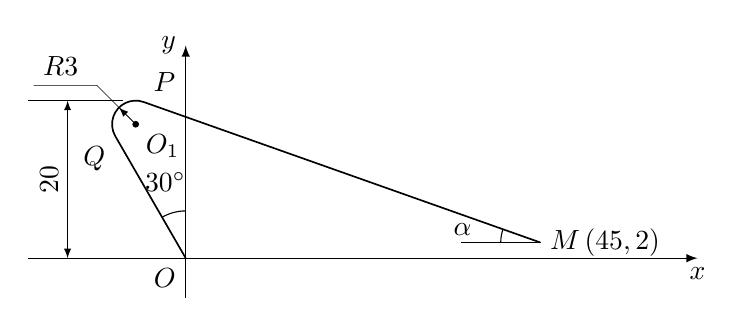
\begin{tikzpicture}[>=latex,scale=0.1]
  \draw[thin,->](-20,0)--(65,0)node[below]{$x$};
  \draw[thin,->](0,-5)--(0,27)node[left]{$y$};
  \tkzDefPoints{0/0/O,0/6/A,1/17/B,-1/17/C,45/2/M,35/2/M'}
  \tkzDefShiftPoint[O](30:3){D}
  \tkzInterLL(A,D)(B,C)\tkzGetPoint{O1}
  \tkzDefShiftPoint[O1](3,0){R}
  \tkzDefLine[tangent from=O](O1,R)\tkzGetPoints{Q}{Q'}
  \tkzDefLine[tangent from=M](O1,R)\tkzGetPoints{P'}{P}
  \tkzDrawArc[semithick](O1,P)(Q)
  \tkzDrawSegments[semithick](O,Q M,P)
  \tkzDrawPoints[fill=black](O1)
  \tkzMarkAngle[size=5](P,M,M')
  \tkzLabelAngle[pos=10](P,M,M'){$\alpha$}
  \tkzMarkAngle[size=6](A,O,Q)
  \tkzLabelAngle[pos=10](A,O,Q){\ang{30}}
  \tkzLabelPoints[above right](P)
  \tkzLabelPoints[below left](O,Q)
  \tkzLabelPoint[below right](O1){$O_1$}
  \tkzLabelPoint[right](M){$M\,(45,2)$}
  \draw[very thin] (-8,20)--(-20,20)(M)--(M');
  \draw[very thin,<->](-15,0)--(-15,20)node[midway,sloped,above]{20};
  \draw[very thin,->](O1)--++(135:3);
  \draw[very thin,](O1)--++(135:7)--++(-8,0)node[above right]{$R3$};
\end{tikzpicture}
\end{document}